\documentclass[10pt,conference,compsocconf]{IEEEtran}

\usepackage{hyperref}
\usepackage{graphicx}	% For figure environment


\begin{document}
\title{Applying Machine Learning Regression to detect Higgs Boson}

\author{
  Alessandro Arrigoni, Emiljano Gjiriti, Paul M\"unnich\\
  \textit{Department of Computer Science, EPFL, Switzerland}
}

\maketitle

\begin{abstract}
The detection of the Higgs Boson particle is a classical machine learning task. As the particle decays very fast, not the particle itself is observed but the signature of its decay. Many decay signatures look very similar and it is up to machine learning models to determine whether the signal is a result of the Higgs Boson or another process or particle in the background. In this study, a regression model with a high accuracy to determine the presence of Higgs Boson is developed. After different approaches like linear regression, least squares regression, ridge regression and logistic regression were applied and tested by 4-fold cross validation. With an accuracy of XX\% and a RMSE of XX, the ridge regression was identified as the most successful model.

\end{abstract}

\section{Introduction}

In the first machine learning project, methods learned in the course are applied to implement a model which can determine the presence of Higgs Boson.
The data which was provided by CERN consists of thirty different features registered. After analyzing the available data in a first step, in a second step, the dataset has been preprocessed and finally applied to train different kinds of models with only significant features. 

\section{Data Analysis and Feature Engineering}
\label{sec:Data Analysis}

The raw data provided by CERN consists of thirty features such as particle mass or the number of jets. The training data also consisted a corresponding indication, whether the decay of Higgs Boson was observed - the value, the final model is supposed to predict from the thirty other features. One of the features was identified as a categorial variable indicating the if zero jets, one jet, two jets or three jets were observed. As the number of jets is strongly associated with certain features being measured or not, we decided to split the dataset into four subsets according to the number of jets. As the jet number in each of the subsets is the same, it is insignificant in the corresponding submodel. Therefore, the column indicating the jet number was removed to simplify the model. For each of the four sets, the columns with unmeasured and thus, insignificant features were removed from the respective set to further simplify the model.
\textbf{Table with columns removed from each of the subsets}

Regardless of the jet number, some features were not measured or not measured correctly. These values which are indicated by the value -999 were replaced by the mean of of the supposedly correctly measured values of the corresponding column. To obtain a more balanced model with weights in the same order of magnitude, we standardized the four subsets. 

To identify redundant information carried by different features, we calculated the Pearson correlation coefficient for every possible combination of two features in all of the four subsets. An absolute value above 0.8 was considered to indicate a high correlation \textbf{source?}. To further simplify the model, one of the two correlating columns was removed from the subsets. 
\textbf{Table with columns removed from each of the subsets due to the correlation coefficient}


\section{Models}
\label{sec:models}

To identify the best method for the detection of Higgs Boson among the methods learned in machine learning, we implemented six different regression methods. We implemented two functions for \textbf{linear regression} using either gradient descent (GD) or stochastic gradient descent (SGD), two functions using normal equations for \textbf{least squares regression} and \textbf{ridge regression}, and two functions for \textbf{logistic regression} and \textbf{regularized logistic regression} using GD.

For the \textbf{hyper-parameter tuning}, we applied a grid search. The grid search can be applied to either minimize the loss function or to maximize the accuracy of the prediction. As we're targeting a model that accurately labels data with either 1 or -1, we optimized the hyper-parameters with respect to achieve the maximum accuracy. 

The \textbf{Least Square} method was the first method examined. The solution of the \textbf{Least Square} problem consists in solving the normal equations, a system of linear equations. By increasing the polynomial degree, powerful models were obtained. To enhance the numerical performance, GD and SGD approaches were tested. GD and SGD methods are based on the gradient of the loss function which is iteratively used to minimze the loss function and to reach a minimum. In contrast to the GD, which calculates the gradient using the whole dataset, the SGD uses stochastic batches of training points and thus, is less computationally demanding. The weights for the SGD are calculated iteratively by the update rule in equation \ref{eq:sgd}.

\begin{equation}
\label{eq:sgd}
w^{t+1} = w^{t} - \lambda  \bigtriangledown _{n} (w^{t})
\end{equation}

With an RMSE of 0.81 instead of 0.8, the results of the GD methods were similarly accurate compared to the Least Square method.
However, by examining the models with cross validation, it turned out that the linear regression models are facing overfitting already by degree 3-4.

To obtain a more solid and powerful model, we implemented a \textbf{ridge regression} based on the normal equations. The standard Euclidean norm ($L_{2}$) was used as a standardizer. The main advantage of the ridge regression is the penalization of large model weights. The result of the ridge regression applying the normal equation is obtained by equation \ref{eq:ridge}. It should be noted that the Least Squares solution is the same formula with $\lambda=0$.

\begin{equation}
\label{eq:ridge}
w_{ridge}^{*}=(X^{T}X+2N\lambda)^{-1}X^{T}y
\end{equation}

In the grid search for ridge regression, we identified a degree of 11 as the optimal degree for the polynomial bases of all subsets. The RMSE of the cross validation was observed to be very high in this case which indicates overfitting. However, as the target of the model development is to maximize the label accuracy (1 or -1), the optimization of the accuracy was the objective of the grid search. 

\textbf{Table with the optimal lambda and d for all subsets}

The target value of the model is binary. Therefore it is very likely to apply the \textbf{Logistic Regression}. This method employs the sigmoid function which returns a value between 0 and 1 indicating the probability that a given number is 1.

The \textbf{Regularized Logistic Regression} is based on the same working principle adding a regularization/penalty term to penalize large weights. Once the weights of the regression are determined, we can predict the probability for each data point in the test set to belong to either 0 or 1 (which can easily converted to -1 and 1 afterwards).

\section{Results}
\label{sec:results}

\section{Discussion}
\label{sec:discussion}



%\subsection{Figures and Tables}
%
%\begin{figure}[tbp]
%  \centering
%  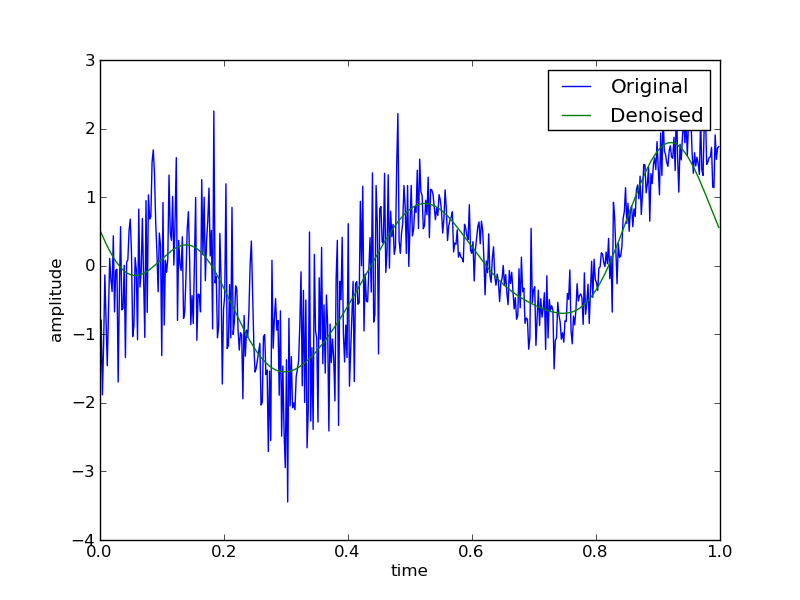
\includegraphics[width=\columnwidth]{denoised_signal_1d}
%  \caption{Signal compression and denoising using the Fourier basis.}
%  \vspace{-3mm}
%  \label{fig:denoise-fourier}
%\end{figure}
%\begin{figure}[htbp]
%  \centering
%  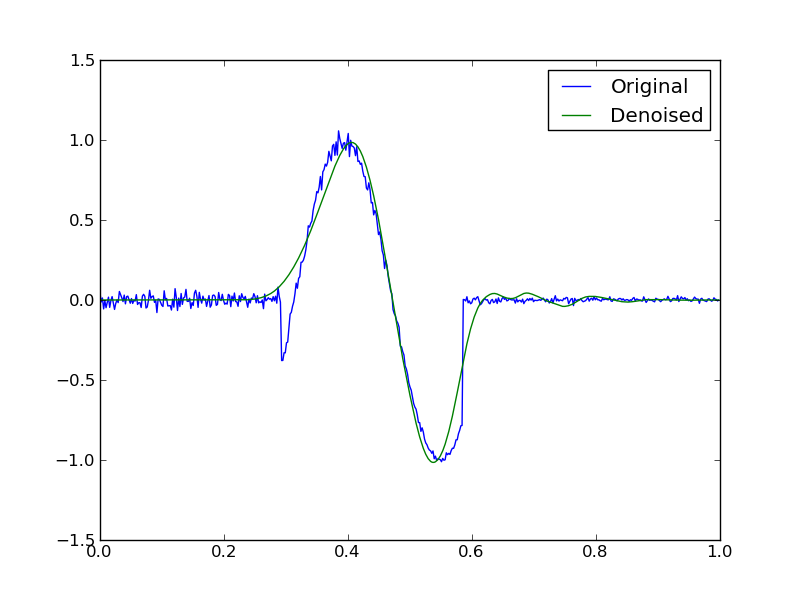
\includegraphics[width=\columnwidth]{local_wdenoised_1d}
%  \vspace{-3mm}
%  \caption{Signal compression and denoising using the Daubechies wavelet basis.}
%  \label{fig:denoise-wavelet}
%\end{figure}


%\begin{table*}[htbp]
%  \centering
%  \begin{tabular}[c]{|l||l|l|l|}
%    \hline
%    Basis&Support&Suitable signals&Unsuitable signals\\
%    \hline
%    Fourier&global&sine like&localized\\
%    wavelet&local&localized&sine like\\
%    \hline
%  \end{tabular}
%  \caption{Characteristics of Fourier and wavelet basis.}
%  \label{tab:fourier-wavelet}
%\end{table*}

\
%\subsubsection{Equations}
%
%There are three types of equations available: inline equations, for
%example $y=mx + c$, which appear in the text, unnumbered equations
%$$y=mx + c,$$
%which are presented on a line on its own, and numbered equations
%\begin{equation}
%  \label{eq:linear}
%  y = mx + c
%\end{equation}
%which you can refer to at a later point (Equation~(\ref{eq:linear})).

%\subsubsection{Tables and Figures}
%
%Tables and figures are ``floating'' objects, which means that the text
%can flow around it.
%Note
%that \texttt{figure*} and \texttt{table*} cause the corresponding
%figure or table to span both columns.



\section{Discussion \\REFERENCES}
\label{sec:discussion}

\bibliographystyle{IEEEtran}
\bibliography{literature}

\end{document}
